\documentclass{article}
\usepackage[a4paper, total={6in, 8in}]{geometry}
\usepackage{amsmath} 
\usepackage{graphicx}
\graphicspath{ {images/} }

\title{Analyzing the choice of transportation}
\author{Elie Daher}

\begin{document}
\pagenumbering{gobble}
\maketitle
\abstract This document contains the problem of analysing the choice of transportation. This problem is from the chapter UTA Methods of the Book: Multiple Criteria Decision Analysis. This document was made during my internship at LAMSADE in the summer of 2017.\\

A DM wants to analyse the choice of transportation. The DM is interstered in the following criteria 
\begin{enumerate}
\item price
\item time (min)
\item comfort (possibility to have a seat)
\end{enumerate}\leavevmode
The evaluation of the previous criteria is presented in the following table: 
\begin{center}
\begin{tabular}{ |c|c|c|c|c| } 
\hline
Means of transportation & Price & Time & Comfort & Ranking of the DM \\
\hline
RER & 3 & 10 & + & 1 \\
METRO (1) & 4 & 20 & ++ & 2 \\
METRO (2) & 2 & 20 & 0 & 2 \\
BUS & 6 & 40 & 0 & 3 \\
TAXI & 30 & 30 & +++ & 4 \\
\hline
\end{tabular}
\end{center}
DM's preferences: $ RER \succ  Metro1 \approx Metro2  \succ  Bus \succ  Taxi$\\
\newpage
First of all, we should specify the scale \footnote{the interval $[g_{i*}, g_{i}^{*}]$ is cut into equal intervals} for each criteria.
\begin{itemize}
\item Price  $\quad \rightarrow \quad [30, 16, 2]$
\item Time  $\quad \rightarrow \quad [40, 30, 20, 10]$
\item Comfort  $\quad \rightarrow \quad [0, +, ++, +++]$
\end{itemize}
According to this formula: $v(g(a)) = \sum_{i=1}^{n} v_i (g_i (a))$ , the value of each alternative may be written: 
\begin{itemize}
\item $v[g(RER)]= 0.07  v_1 (16) + 0.93 v_1(2) + v_2(10) + v_3(+)$
\item $v[g(METRO1)]= 0.14 v_1 (16) + 0.86 v_1(2) + v_2(20) + v_3(++)$
\item $v[g(METRO2)]= v_1 (2) + v_2(20) + v_3(0) =  v_1 (2) + v_2(20) $
\item $v[g(BUS)]= 0.29  v_1 (16) + 0.71 v_1(2) + v_2(40) + v_3(0) = 0.29 v_1 (16) + 0.71 v_1(2)$
\item $v[g(TAXI)]= v_1 (30) + v_2(30) + v_3(+++) = v_2(30) + v_3(+++)$
\end{itemize}
We have that $v_1(30) = v_2(40) = v_3(0) = 0$. \\
Since the marginal value $u_i(g_i)$ can be expressed in terms of variables $w_{ij}$: $u_i(g_i^{j}) = \sum _{t=1}^{j-1} w_{it}$ , the value of each alternative can be written: 
\begin{itemize}
\item $v[g(RER)]= w_{11} + 0.93 w_{12} + w_{21} + w_{22} + w_{23} + w_{31}$
\item $v[g(METRO1)]=w_{11} + 0.86 w_{12} + w_{21} + w_{22} + w_{31} + w_{32}$
\item $v[g(METRO2)]= w_{11} + w_{12} + w_{21} + w_{22} $
\item $v[g(BUS)]= w_{11} + 0.71 w_{12}$
\item $v[g(TAXI)]= w_{21} + w_{31} + w_{32} + w_{33}$
\end{itemize}
For each pair of consecutive alternatives, we express the difference between them: 
\begin{itemize}
\item $\Delta (RER, METRO1) = 0.07 w_{12} + w_{23} - w_{32} \geq \delta$
\item $\Delta (METRO1, METRO2) = -0.14 w_{12} + w_{31} + w_{32}  = 0$
\item $\Delta (METRO2, BUS) = 0.29 w_{12} + w_{21} + w_{22} \geq \delta$
\item $\Delta (BUS, TAXI) = w_{11} + 0.71w_{12} - w_{21} - w_{31} - w_{32} - w_{33} \geq \delta$
\end{itemize}
Having $\delta = 0.05$, we can solve the following LP:\\

Objective:  
\begin{equation}
	Minimize \quad \sum_{a \in A} \sigma _{a}^{+} + \sigma _{a}^{-}
\end{equation}

Subject to: \\
\begin{equation}
	\begin{cases}
		0.07 w_{12} + w_{23} - w_{32}  -\sigma _{RER}^{+} +\sigma _{RER}^{-} +\sigma _{METRO1}^{+} - \sigma _{METRO1}^{-}\geq \delta\\
		-0.14 w_{12} + w_{31} + w_{32}  -\sigma _{METRO1}^{+} +\sigma _{METRO1}^{-} +\sigma _{METRO2}^{+} - \sigma _{METRO2}^{-} = 0  \\
		 0.29 w_{12} + w_{21} + w_{22}  -\sigma _{METRO2}^{+} +\sigma _{METRO2}^{-} +\sigma _{BUS}^{+} - \sigma _{BUS}^{-} \geq \delta\\
		w_{11} + 0.71w_{12} - w_{21} - w_{31} - w_{32} - w_{33} -\sigma _{BUS}^{+} +\sigma _{BUS}^{-} +\sigma _{TAXI}^{+} - \sigma _{TAXI}^{-} \geq \delta\\
		w_{11} + w_{12} + w_{21} + w_{22} + w_{23} + w_{31} + w_{32} + w_{33} = 1\\

	\end{cases}
\end{equation}
So by using the com.google.ortools library, we can solve the Linear Program above with $\sigma = 0.05$. This Linear Program solution is coded in Java class ChoiceTransportation.\\
By executing the class ChoiceTransportation, you will have the following result: \\
\begin{center}
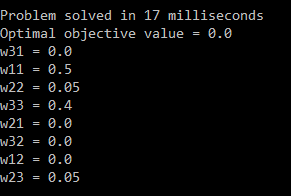
\includegraphics[height=5cm]{result.png}
\end{center}
An optimal solution is $w_{11} = 0.5$, $w_{22} = 0.05$, $w_{23} = 0.05$, $w_{33} = 0.4$ with $\sum_{a \in A} \sigma _{a}^{+} + \sigma _{a}^{-} = 0$. The utilities found for each alternative are as follows: \\ 
\begin{itemize}
\item $v(g(RER)) = 0.6$
\item $v(g(METRO1)) = 0.55$
\item $v(g(METRO2)) = 0.55$
\item $v(g(BUS)) = 0.5$
\item $v(g(TAXI)) = 0.4 $
\end{itemize}
Those utilities are consistent with the DM's preference ranking. \\

\end{document}